% latexmk -pvc -pdf slides.tex
\documentclass{beamer}

\beamertemplatenavigationsymbolsempty

% literatur
\usepackage[backend=biber,style=alphabetic]{biblatex}

\addbibresource{../util/literature.bib}

\usepackage{../util/zariski}

\usepackage{csquotes}
\usepackage{cancel}
\usepackage{tabularx}
\usepackage{hyperref}
\usepackage{tikz}
\usetikzlibrary{cd,arrows,shapes,calc,through,backgrounds,matrix,trees,decorations.pathmorphing,positioning,automata}
\usepackage{graphicx}
\usepackage{color}

\usepackage{mathpartir}
\newcommand{\yields}{\vdash}
\newcommand{\cbar}{\, | \,}

\newcommand{\nop}[1]{\textcolor{bg}{#1}}


% für tabellen
\usepackage{booktabs}

\title{Synthetic Algebraic Geometry and Synthetic Stone Duality}
\date{August 7, 2025}

\begin{document}

\begin{frame}
  \titlepage
\end{frame}

\begin{frame}
  This and related work is and was done by:
  \begin{center}
    \begin{tabularx}{\textwidth}{XXX}
      Peter Arndt & Reid Barton & Ulrik Buchholtz \\
      Ingo Blechschmidt & Felix Cherubini & Johan Commelin \\
      Thierry Coquand & Fabian Endres & Freek Geerligs \\
      Jonas Höfer & Tim Lichtnau & Hugo Moeneclaey \\
      David Jaz Myers & Marc N-W & Armaan Rashid \\ 
      Matthias Ritter & Christian Sattler & Lukas Stoll \\
      David Wärn & Mark Williams &
    \end{tabularx}
  \end{center}
  \pause
  Early work of Felix Cherubini on the project was sponsored by The United States Air Force Research Laboratory under agreement number FA9550-15-1-0053.
\end{frame}

\begin{frame}
  Work I will describe in the following was done by:
  \begin{center}
    \begin{tabularx}{\textwidth}{XXX}
      \nop{Peter Arndt} & \nop{Reid Barton} & \nop{Ulrik Buchholtz} \\
      Ingo Blechschmidt & Felix Cherubini & \nop{Johan Commelin} \\
      Thierry Coquand & \nop{Fabian Endres} & Freek Geerligs \\
      \nop{Jonas Höfer} & \nop{Tim Lichtnau} & Hugo Moeneclaey \\
      \nop{Marc N-W} & Armaan Rashid & Matthias Ritter \\ 
      \nop{Christian Sattler} & \nop{Lukas Stoll} & David Wärn \\
      \nop{Mark Williams} & &
    \end{tabularx}
  \end{center}
\end{frame}

\begin{frame}
  A more complete overview is at \url{https://github.com/felixwellen/synthetic-zariski}:
  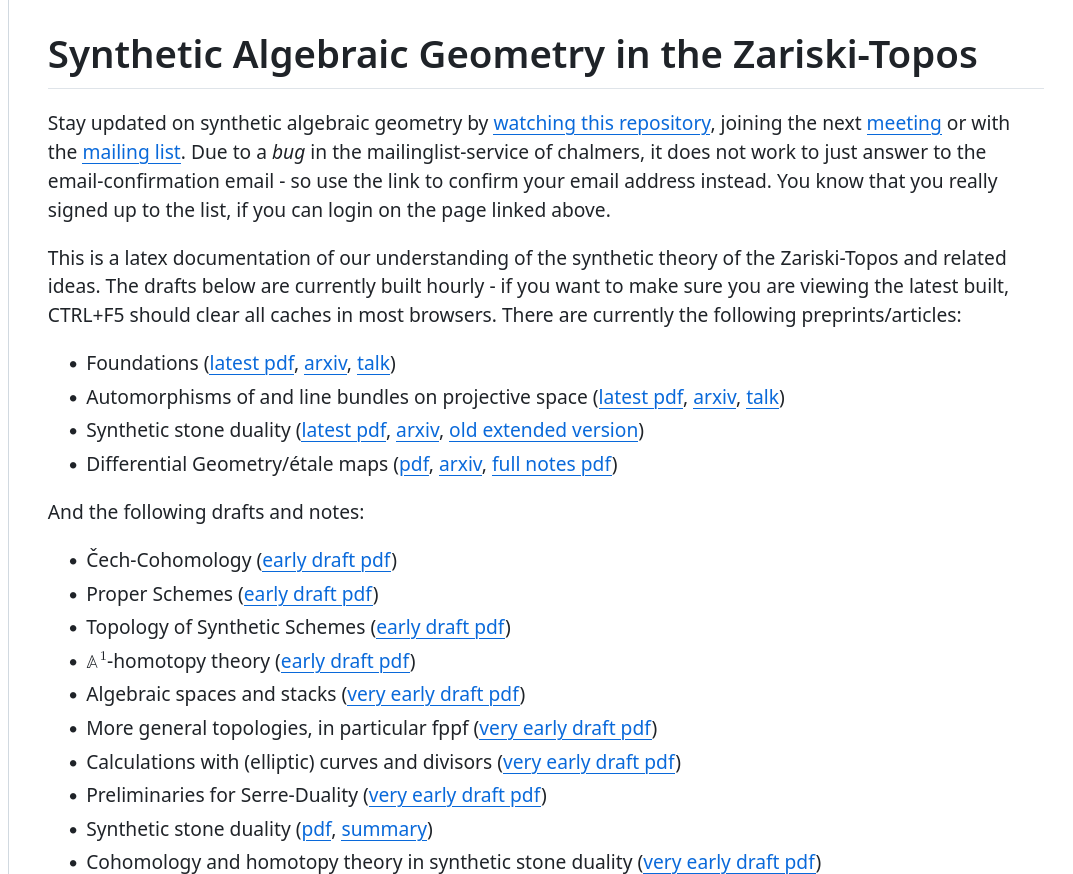
\includegraphics[width=\textwidth]{repo.png}
\end{frame}

\begin{frame}
  \vspace{1cm}
  \begin{center}
    \begin{tikzpicture} 
      [ 
      node distance=.8cm, 
      circled/.style={draw, ellipse, ultra thick, fill=blue!12},
      edge from parent/.style={very thick,draw=black,-latex},
      plaintext/.style={}
      ]

      \tikzstyle{level 1}=[sibling angle=81,level distance=4cm]

      \node[circled] (hott) {HoTT+Data+Axioms} [counterclockwise from=207]
      child { 
        node[circled] (grp) {$\infty$-Groupoids} 
        edge from parent [-latex] node (grp) 
        {
          \begin{tikzpicture}[scale=0.8, rotate=25]
            \draw[-, red, ultra thick] (0,0) to (1,1);
            \draw[-, red, ultra thick] (1,0) to (0,1);
          \end{tikzpicture}
        } 
      }
      child { node[matrix, circled, inner sep=0pt] (smgrp) 
        {
          \node[circled, minimum height=0.7cm, minimum width=3cm] (mfd) {Schemes};
          \node[below of=mfd, text width=3cm,
          node distance=0.9cm] 
          {``Constructive Zariski-sheaves''}; \\
        }
      }
      ;
    \end{tikzpicture}
  \end{center}
  \vspace{1cm}
  {\footnotesize * Schemes = quasi-compact, quasi-separated schemes of finite presentation}
\end{frame}

\begin{frame}
  \frametitle{\textbf{Synthetic Algebraic Geometry}}
  \pause
  $R$ is a commutative ring. \\
  \vspace{0.4cm}
  \pause

  $V:= \{(x,y):R^2\mid x^2+y^2=1 \}$ \\

  \pause
  Adding equations like $0=0$, $x(x^2+y^2)=x$ does not change the type $V$. \\
  \pause
  $V$ is determined by the $R$-algebra $A:= R[X,Y]/(X^2+Y^2-1)$.
  \pause
  We can recover it: $V=\Hom_{\Alg{R}}(A,R)$. \\
  \vspace{0.4cm}
  \pause
  \begin{definition}
    \begin{enumerate}[(i)]
    \item An $R$-algebra is finitely presented (fp) if it is merely $R[X_1,\dots,X_n]/(P_1,\dots,P_l)$.
    \item $\Spec(A):= \Hom_{\Alg{R}}(A,R)$ is the \emph{spectrum} of an fp $R$-algebra $A$.
    \item Any $X$ such that there is an $A$ with $X=\Spec(A)$ is called \emph{affine scheme}.
    \end{enumerate}
  \end{definition}
\end{frame}

\begin{frame}
  \frametitle{The 3 Axioms of SAG}
    \textbf{Axiom (Duality):}
    The map
    \begin{align*}
      A \to R^{\Spec A} \\
      a\mapsto (\varphi\mapsto \varphi(a))
    \end{align*}
    is an equivalence
    for any finitely presented $R$-algebra $A$. \\
  \pause
  \vspace{5mm}
  \textbf{Axiom (Locality):} The ring $R$ is local:
  $1\neq 0$ and for all $x,y:R$ such that $x+y$ is invertible, $x$ is invertible or $y$ is invertible.
  
  \vspace{5mm}
  \textbf{Axiom (Zariski-local choice):}\\
  For every surjective $\pi$, there merely exist local sections $s_i$
  with $f_1, \dots, f_n : A$ such that $(f_1,\dots,f_n)=(1)$.
\end{frame}

\begin{frame}
  \frametitle{\textbf{Synthetic Algebraic Geometry}}
  A proposition $P$ is \textbf{open} if there merely are $r_1,\dots,r_n:R$
  such that
  \[ P \Leftrightarrow r_1\neq 0 \vee \dots \vee r_n\neq 0\]
  \pause
  ($r\neq 0 \Leftrightarrow r\text{ invertible}$) \\
  \pause
  $U\subseteq X$ is open if $x\in U$ is an open proposition for all $x:X$. \\
  \pause
  \textbf{Example:} $\{x:R\mid x\neq 0\}$ and $\{x:R\mid x\neq 1\}$ are open subsets. By locality, they cover $R$. \\
  \vspace{5mm}
  \pause
  By Zariski-local choice every open $U\subseteq \Spec(A)$ is a finite union of subsets of the form ($f:\Spec(A)\to R$)
  \[ D(f) := \{x:\Spec(A) \mid f(x)\neq 0 \} \] \\
  \pause
  A type $X$ is a \textbf{scheme} if
  there exist open $U_1, \dots, U_n \subseteq X$
  such that $X = \bigcup_i U_i$
  and every $U_i$ is an affine scheme. \\
  \vspace{5mm}
  \pause
  \textbf{Morphisms} of schemes are just maps between types.
  
\end{frame}

\begin{frame}
  \begin{columns}
    % Rechte Spalte mit Bild
    \begin{column}{0.5\textwidth}
      \textbf{Projective Space} $\bP^n$ \\
      \pause
      ($n\geq 1$)
      \vspace{4mm}
      \pause
      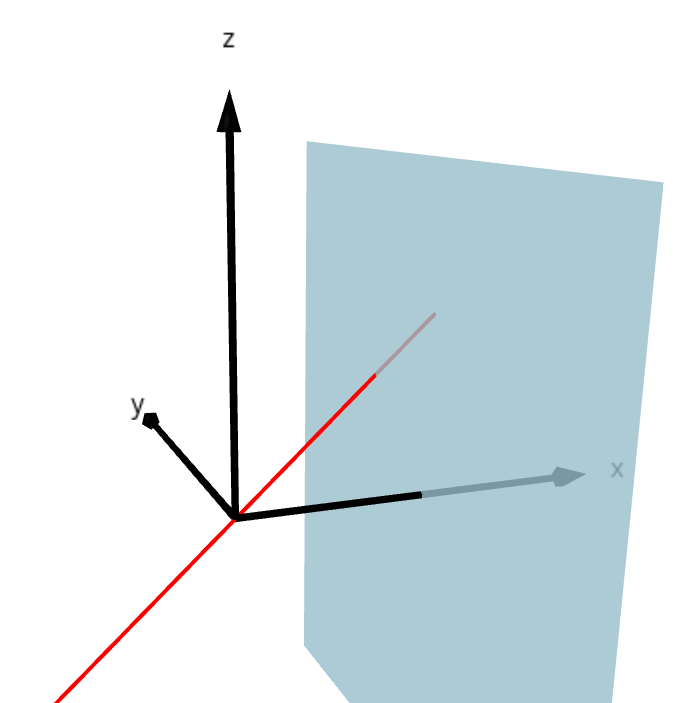
\includegraphics[width=\textwidth]{projective-space.png}
      \vspace{2cm}
    \end{column}
    
    % Linke Spalte mit Text
    \begin{column}{0.5\textwidth}
      \pause
      Points are straight lines through the origin in $R^{n+1}$.
      \[ \bP^n:= R^{n+1}\text{\textbackslash}\{0\}/\sim \]
      where $x\sim y \Leftrightarrow \exists \lambda :R. x=\lambda y$. 

      \vspace{1em}
      \pause
      \textbf{Or:}
      \[ \bP^n:= \sum_{l:\mathrm{Lines}}l^{n+1}\text{\textbackslash}\{0\} \]
      where
      \[\mathrm{Lines}=\{L:\Mod{R}\mid \|L=R^1\|\}\]
      \pause
      Projective space is a scheme with cover
      \[ U_i([x]) := \text{($x_i$ is invertible)}. \]      
    \end{column}
  \end{columns}
\end{frame}


\begin{frame}
  \frametitle{Properties of Projective Space}
  All functions $\bP^n\to R$ are constant. ($\implies$ $\bP^n$ is not affine.) \\  
  \pause
  \vspace{4mm}
  \begin{columns}
    \begin{column}{0.42\textwidth}
  \textbf{Proof:} (Start with $n=1$) 
  \[
\begin{tikzcd}[ampersand replacement=\&, column sep=small]
    R^\times \ar[r,"\frac{1}{x}"]\ar[d,swap,"x"] \& R^1 \ar[d] \\
    R^1 \ar[r] \& \bP^1
\end{tikzcd}
\]
\pause
Algebra $\implies$ Any $\bP^1\to R$ is constant. \\
\pause
Details: A map $\bP^1\to R$ corresponds to polynomials $f,g:R^1\to R$ such that $f(x)=g(\frac{1}{x})$, so $f=g$ is constant.
      
    \end{column}
    \begin{column}{0.48\textwidth}
      \pause
      ($n>1$) \\
      \pause
      Idea: For $x,y:\bP^n$, find a line ($=\bP^1$) through $x,y$, then $f(x)=f(y)$. \\
      \pause
      This actually needs a third point to work:
      \pause
      \vspace{5mm}
      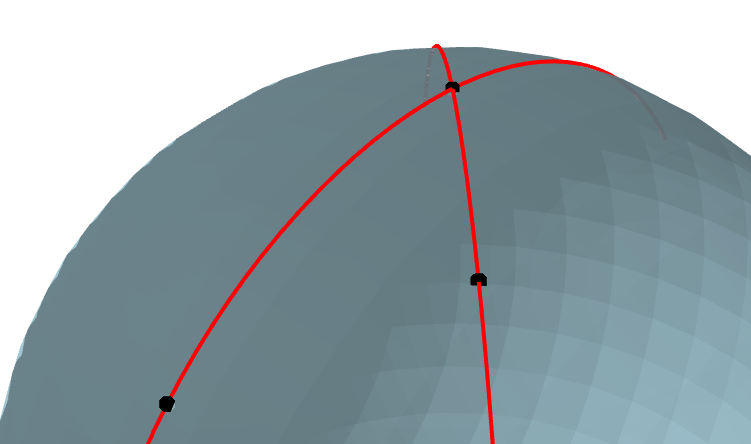
\includegraphics[width=\textwidth]{projective-space2.png}
    \end{column}
  \end{columns}
\end{frame}

\begin{frame}
  \frametitle{Properties of Projective Space}
  A \textbf{line bundle} on a type $X$ is a map $\mathcal L:X\to \mathrm{Lines}$.
  Note that $\mathrm{Lines}=K(R^\times,1)$.\\
  \vspace{4mm}
  \pause
  \textbf{Theorem:} $(\bP^n\to \mathrm{Lines}) = \Z\times K(R^\times,1)$. \\
  \pause
  \textbf{Or:} Each line bundle on $\bP^n$ is merely one of the following:
  \begin{enumerate}[(i)]
  \item $\mathcal O(-1):=(([x] : \bP^n) \mapsto \text{ $R\langle x\rangle : \mathrm{Lines}$})$
  \item $\mathcal O(-d):=\mathcal O(-1)^{\otimes d}$ for $d:\N$.
  \item $\mathcal O(d):=(x\mapsto \Hom_{\Mod{R}}(\mathcal O(-d)_x,R))$.
  \end{enumerate}
  \vspace{4mm}
  \pause
  Any open $U\subseteq \bP^n$ is a finite union of more general
  \[ D(f):=\{x:\bP^n\mid f(x)\neq 0 \}\]
  with $f:(x:\bP^n)\to \mathcal O(d)_x$ for some $d:\N$.
\end{frame}

\begin{frame}
  \frametitle{Projective Schemes}
  \pause
  A scheme $X$ is \textbf{projective} if it merely is a closed subset of some $\bP^n$. \\
  \vspace{4mm}
  \textbf{Example and tentative definition:}
  An elliptic curve is a pointed projective scheme $C$
  which is smooth of dimension $1$, connected and $H^1(C,R)=1$.
  \pause
  Assume $2\neq 0,3\neq 0$ in $R$.
  For all $a,b:R$ such that $4a^3+27b^2\neq 0$ we have the elliptic curve
  \[ E_{a,b}:=\{ [x,y,z] :\bP^2\mid y^2z-x^3-axz^2-bz^3=0 \}.\] \\
  \pause
  \textbf{Classically}, over a field $k$, there is a converse - each elliptic curve is of the above form (if $2\neq 0, 3\neq 0$ in $k$).
  % Silverman, p. 59
  \pause
  There is a proof using the Riemann-Roch theorem, which can be derived from Serre-Duality.
  The latter relies on cohomology computations on $\bP^n$.
\end{frame}

\begin{frame}
  \frametitle{Cohomology of Line Bundles on Projective Space}
\begin{theorem}
  \label{calculate-cohomology-twisting-sheaves}
  \begin{enumerate}[(a)]
  \item \label{calculate-cohomology-twisting-sheaves-a}
  For all $n:\N$, $d:\Z$, there are isomorphisms $R[X_0,\dots,X_n]_d\to H^0(\bP^n,\mathcal O(d))$ of $R$-modules, inducing an isomorphism $R[X_0,\dots,X_n]\to \bigoplus_{d:\Z} H^0(\bP^n,\mathcal O(d))$ of graded $R[X_0,\dots,X_n]$-modules.
  \item \label{calculate-cohomology-twisting-sheaves-b}
        $H^n(\bP^n,\mathcal O(-n-1))=R$ is free of rank 1 and $H^n(\bP^n,\mathcal O(d))=0$ for $d>-n-1$.
  \item \label{calculate-cohomology-twisting-sheaves-c}
    The canonical map given by tensoring
    \[
      H^0(\bP^n,\mathcal O(d)) \times H^n(\bP^n,\mathcal O(-d-n-1))\to R
    \]
    is a perfect pairing of finite free $R$-modules for all $d:\Z$.
  \item $H^i(\bP^n,\mathcal O(d))=0$ for $i\in\{1,\dots,n-1\}$ and all $d:\Z$.
  \end{enumerate}
\end{theorem}
\end{frame}

\begin{frame}
  \frametitle{Serre-Duality for Projective Space}
  Algebraic Geometry textbook by Hartshorne, p.\ 257: 
  \begin{center}
  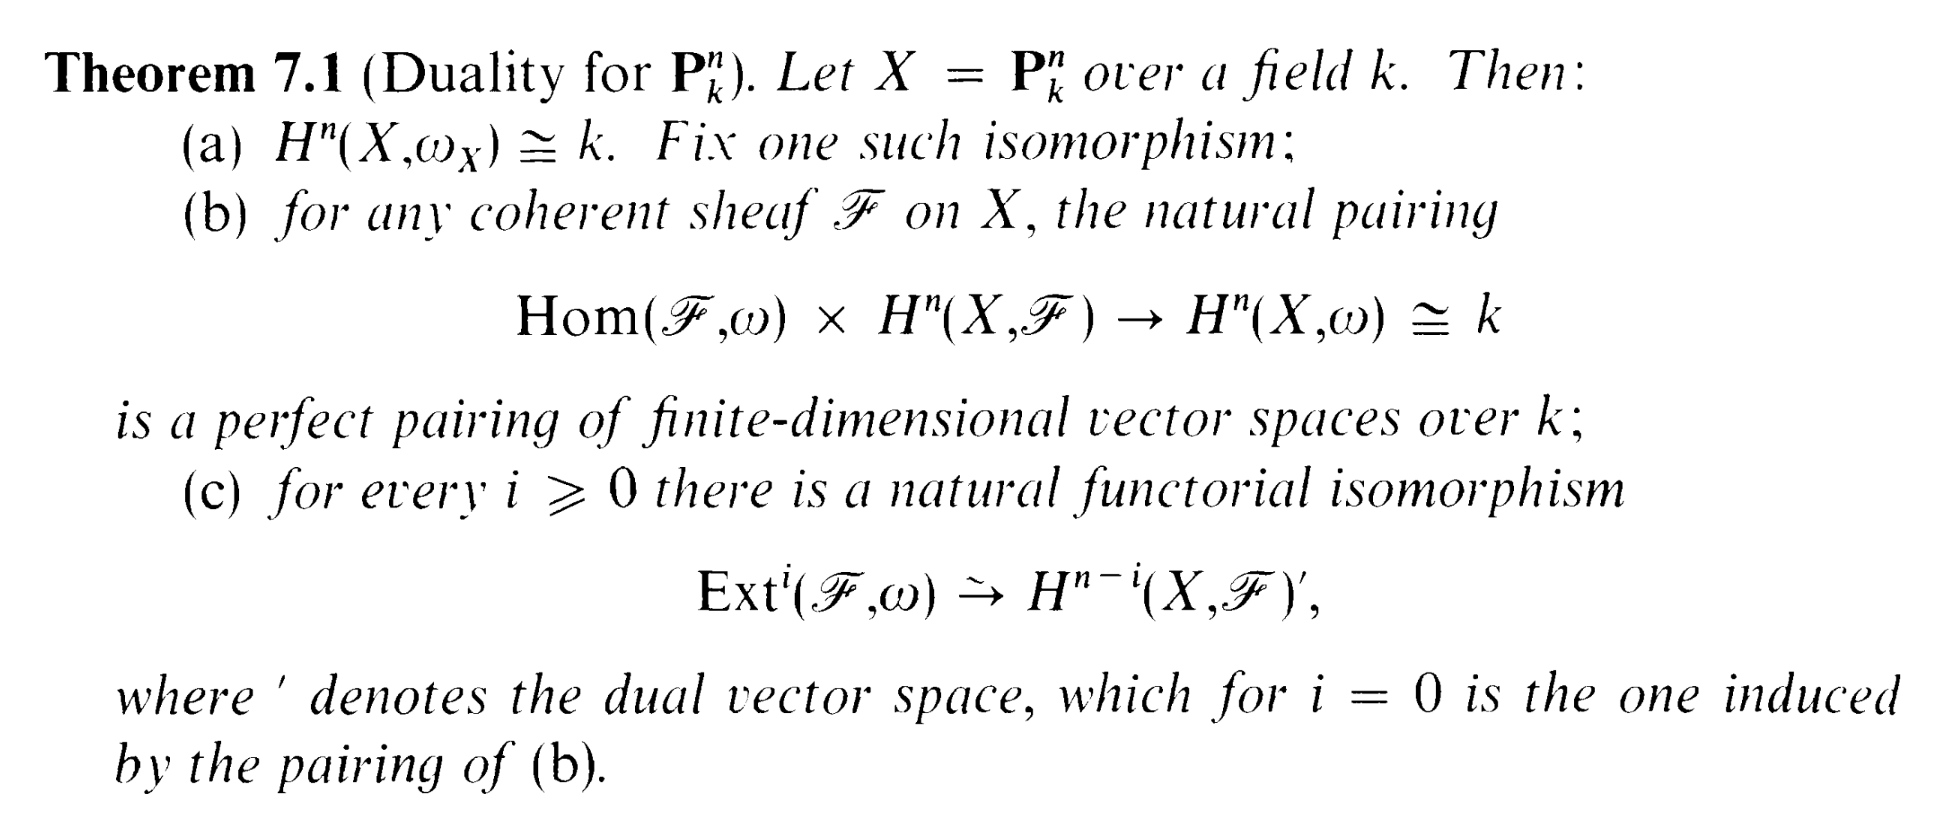
\includegraphics[keepaspectratio,
                                 width=0.8\paperwidth,
                                 height=\paperheight]{hartshorne1.png}    
  \end{center}
  \pause
  \textbf{Challenges:}
  \begin{enumerate}[(i)]
  \item (c) needs that dualization is exact.
  \item It is unclear if we have a good replacement for ``coherent''.
  \item It is even less clear if cohomology groups of coherent sheaves will be coherent - which is needed in (c).
  \end{enumerate}
\end{frame}

\begin{frame}
  \frametitle{Synthetic Stone Duality} 
  Now $\Spec B:\equiv \Hom_2(B,2)$, for $B$ a boolean algebra. \\
  \textbf{Axiom (Duality):} \vspace{-.4cm}
    \begin{align*}
      B \to 2^{\Spec B} \\
      a\mapsto (\varphi\mapsto \varphi(a))
    \end{align*}
    is an equivalence
    for any \emph{countably} presented boolean algebra $B$. \\
  \pause
  \textbf{Axiom (Formal surjections):} \\ %% $\neg\neg\Spec B\Rightarrow ||\Spec B ||$ \\
  $g:B\to C$ injective $\implies$ $(-)\circ g: \Sp(C) \to \Sp(B)$ surjective. \\
  \textbf{Axiom (Depedent choice):}  \\
  For all types $(E_n)_{n:\N}$ with surjections $E_{n+1}\twoheadrightarrow E_n$ for all $n:\N$, the projection from the sequential limit $\lim_kE_k$ to $E_0$ is surjective.
  \textbf{Axiom (Zariski-local choice):}\\
  For every surjective $\pi$, there merely is a surjection $\Spec B'\to \Spec B$
  together with a section $s$:
  \[ \begin{tikzcd}[ampersand replacement=\&, column sep=small]
    \& E \ar[d, two heads, "\pi"] \\
    \Spec B' \ar[r, ->>] \ar[ur, bend left, dashed, "s"] \& \Spec B
  \end{tikzcd} \]
\end{frame}


\begin{frame}
  \frametitle{Constructions, Definitions and Theorems}
  \begin{itemize}
  \item $X$ with $X=\Spec B$ is (called) a \emph{Stone space}. \pause \textbf{Or:} Sequential limit of finite sets. \pause \textbf{Example:} $2^{\mathbb N}$.
    \pause
  \item $ [0,1] :\equiv 2^{\mathbb N}/\sim $ \pause \quad where $0.a_0\dots a_n0\bar{1}\sim 0.a_0\dots a_n1\bar{0}$
    \pause
  \item $A\subseteq X$ is \emph{closed} if $\forall x:X. \exists \alpha:2^{\mathbb N}. V(x)=(\alpha=0)$.
    \pause
  \item A \emph{compact Hausdorff space} is a type $X$ with closed equality types such that there is a surjection $S\to X$ from a Stone space $S$.
    \pause
  \item Open subsets of $[0,1]$ are exactly countable unions of open intervals. It is also compact, connected and we have $H^1([0,1],\mathbb Z)=0$.
    \pause
  \item $L_{[0,1]}\mathbb S^1=S^1$ for $L_{[0,1]}$ the nullification at $[0,1]$.
    \pause
  \item Brouwer's fixed-point theorem and Borsuk-Ulam are provable using synthetic homotopy theory.
    \pause
  \item $H^n(\mathbb I, A)=0$, $n>0$, $A$ fp abelian.
    \pause
  \item $K(A, n)$ is $L_{[0,1]}$-modal. 
  \item Any finite homotopical CW complex $X_{h}$ which is the limit of its Postnikov-tower is $L_{[0,1]}$-modal. \pause Then: $L_{[0,1]}X_{\mathrm{Top}}=X_h$.
  \end{itemize}
\end{frame}

\begin{frame}
  \begin{center}
    Thank you!
  \end{center}
\end{frame}
\end{document}
